\section{\textcolor{black}{Current work and future considerations}}


\begin{frame}
\frametitle{Application on PISA pile}
\centering
\only<1>{
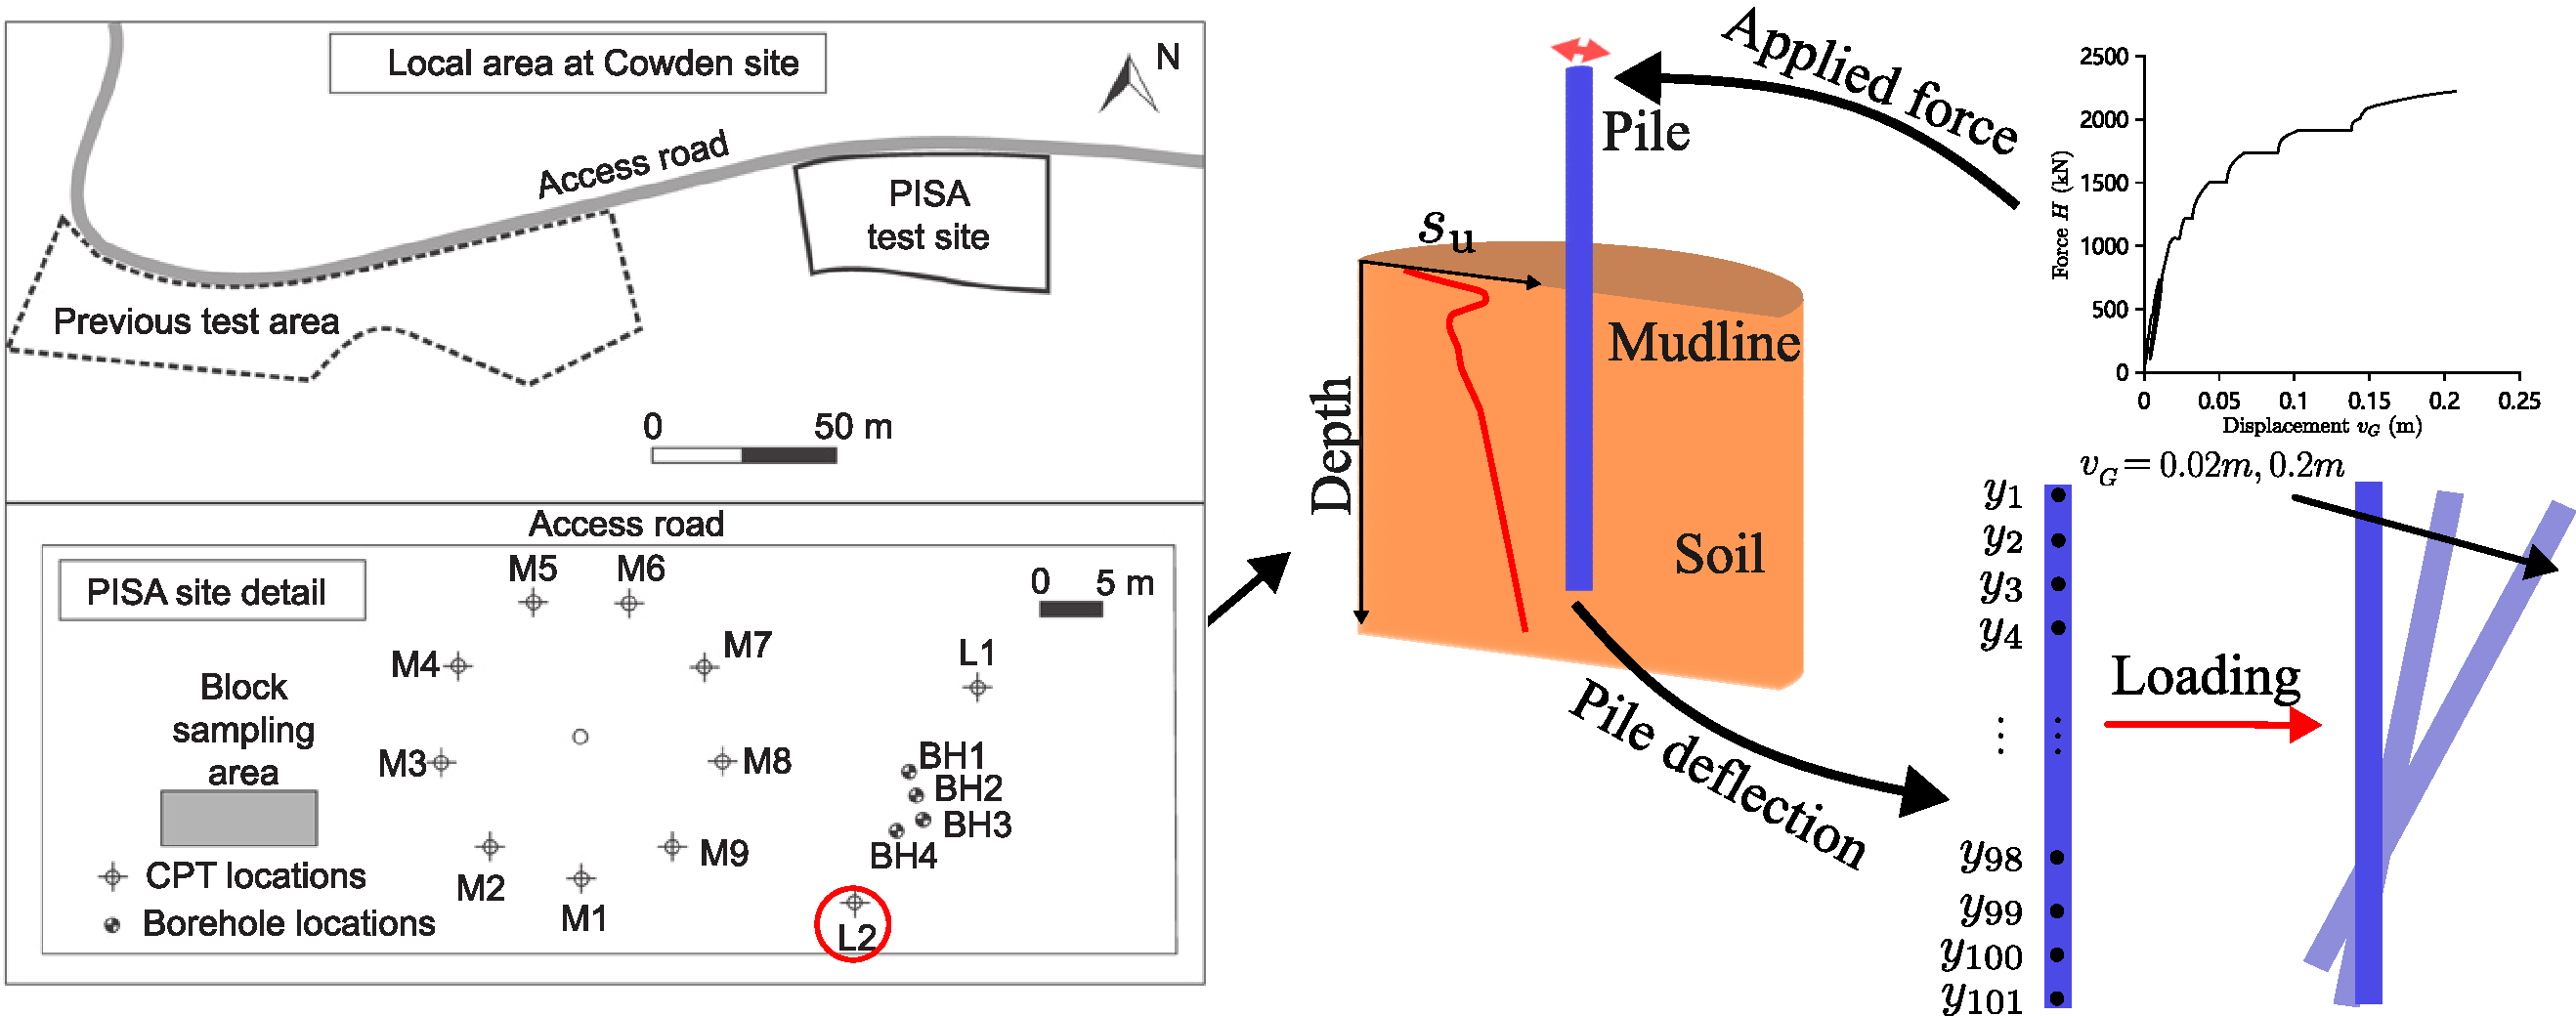
\includegraphics[scale=0.3]{figures/figure-pisapile.pdf}
}
\only<2>{
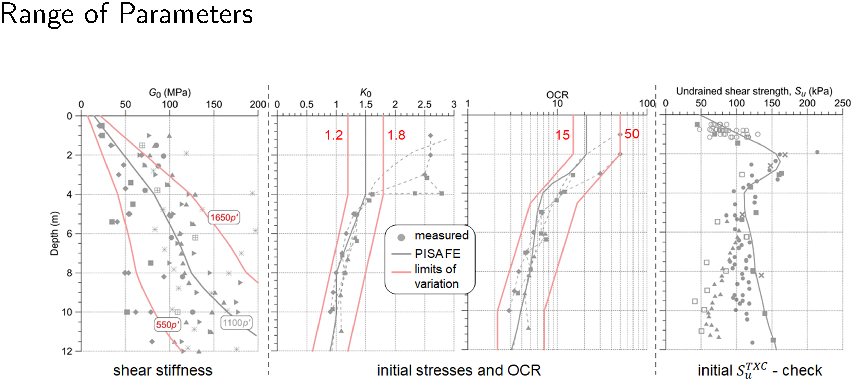
\includegraphics[scale=1]{figures/figure-pisa_parameter_range.pdf} \tiny\footcite{zdravkovic2024}
}
\only<3>{
\centering
\begin{adjustbox}{width=10cm}
\begin{tikzpicture}[%
				x=1.0cm, y=0.6cm,
				every node/.style={
					text height=1ex,
					text depth=.25ex,
				},]
				
				% nodes
				\node[main,line width = 1.5pt] (x0) {$y_{0}$};%
				\node[main,above=of x0,fill=black!10] (y0) {$x_{0}$}; %
				\node[right=of y0] (dotsy) {$\dots$};
				\node[main, right= of dotsy,fill=black!10] (y-1) {$x_{t-1}$}; %
				\node[main, below= of y-1,line width = 1.5pt] (x-1) {$y_{t-1}$};%
				\node[main, right= of x-1,line width = 1.5pt] (x) {$y_{t}$};%
				\node[main, right= of y-1,fill=black!10] (y) {$x_{t}$}; %
				\node[main, right= of x,line width = 1.5pt] (x+1) {$y_{t+1}$};%
				\node[main, right= of y,fill=black!10] (y+1) {$x_{t+1}$}; %			
				\node[right=of y+1] (dotsy2) {$\dots$};	
				
				\node[below=of x0] (prior) {\color{blue} Prior};
				\node[below=of x-1] (obs) {\color{blue} Observations, $\mathcal{Y}$};
				\node[above=of y] (main) {\color{blue}Latent states};
				\node[above=of y0] (initial) {\color{blue} Initial latent state};

				% edges 
				\edgex {y0} {x0}; %
				\edgex {y0} {dotsy}; %
				\edgex{dotsy} {y-1} ; %
				\edgex {y-1} {x-1}; %
				\edgex {y} {x}; %
				\edgex {y-1} {y}; %				
				\edgex {y} {y+1}; %
				\edgex {y+1} {x+1}; %
				\edgex {y+1} {dotsy2}; %
				
				\draw [->,blue] (prior) to[out=+100,in=-70] (x0);
				\draw [->,blue] (obs) to[out=+60,in=-70] (x-1);
				\draw [->,blue] (obs) to[out=+60,in=-70] (x);
				\draw [->,blue] (obs) to[out=+60,in=-70] (x+1);
				
				\draw [->,blue] (main) to[out=-60,in=+70] (y-1);
				\draw [->,blue] (main) to[out=-60,in=+80] (y);			
				\draw [->,blue] (main) to[out=-60,in=+90] (y+1);					
				\draw [->,blue] (initial) to[out=-60,in=+90] (y0);				
				%label
				\end{tikzpicture}
    \end{adjustbox}
}
\only<4>{
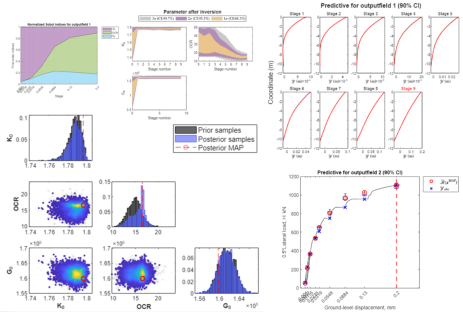
\includegraphics[scale=1.4]{figures/figure-pisa_results.pdf}
}
\end{frame}



\begin{frame}
\frametitle{Future considerations:}

\begin{enumerate}
\setlength\itemsep{1em}
    \item Careful with aleatoric and epistemic types of uncertainties
 
    \item Four UQ components are equally important

    \item Consider different types of uncertainty into Bayesian inference required linked with likelihood-(\alert{currently doing})

    \item Consider taking actions in digital twin-(\alert{future plan})
\end{enumerate}

    
\end{frame}





